\documentclass[letterpaper, reqno,11pt]{article}
\usepackage[margin=1.0in]{geometry}
\usepackage{color,latexsym,amsmath,amssymb,graphicx,float,listings,tikz}
\usepackage{hyperref}

\hypersetup{
colorlinks=true,
linkcolor=magenta,
filecolor=magenta,
urlcolor=cyan,
}

\graphicspath{ {images/} }

\begin{document}
\pagenumbering{arabic}
\title{ELEC 302 Lab 1 Prelab}
\date{04/02/24}
\author{Xander Naumenko}
\maketitle

{\medskip\noindent\bf Question 1: } Read the description of Tasks 1-3 assigned in these sheets.

Done

{\medskip\noindent\bf Question 2:} Review the lecture notes and the sections in Chapter 3 of the text for the following circuits: half wave rectifier, full wave rectifier using a center tap transformer, and full wave rectifier using a bridge circuit. Find the formula for each circuit to calculate the corresponding filter capacitor. Also review relevant supplementary materials referred to in class.

These formulae can be found in the lecture 5 notes. Assuming nonideal diodes, they are:
\begin{itemize}
    \item {Half wave rectifier: $C=\frac{V_p-V_d}{fR_LV_r}$}
    \item {Center tap full wave rectifier: $C=\frac{V_p-V_d}{2fR_LV_r}$}
    \item {Bridge full wave rectifier: $C=\frac{V_p-2V_d}{2fR_LV_r}$}
\end{itemize}

{\medskip\noindent\bf Question 3:.} Find the data sheets for the rectifier diode and the zener diode listed above.

These can found at the following urls:
\begin{itemize}
    \item{\href{https://www.vishay.com/docs/88503/1n4001.pdf}{https://www.vishay.com/docs/88503/1n4001.pdf}}
    \item{\href{https://media.digikey.com/pdf/Data%20Sheets/EIC%20PDF's/1N5338B-88B.pdf}{https://media.digikey.com/pdf/Data\%20Sheets/EIC\%20PDF's/1N5338B-88B.pdf}}
\end{itemize}

{\medskip\noindent\bf Question 4:} For Task 3, draw the circuit diagram of a 5.1-V Zener voltage regulator. Calculate the resistance coupled in series with the Zener diode so to have a standby (no load) current of 66.7 mA. Assume the input voltage to the regulator is around 15 V.

See figure \ref{fig:q4} and it's caption for the circuit diagram. To size the resistor, $R_L=\infty$ and the zener diode can be modeled as a $1.5\Omega$ resistor (given in it's datasheet above) and a $V_{ZD}$ voltage supply. Again from the datasheet, we have $V_{ZD}=V_Z-Z_{ZT}I_{ZT}=5.1-0.24\cdot 1.5=4.74\text{V}$. Then we have that $R=\frac{V}{I}-Z_{ZT}=\frac{15-4.74}{0.0667}-1.5=152.3\Omega$.

\begin{figure}[htpb]
    \centering
    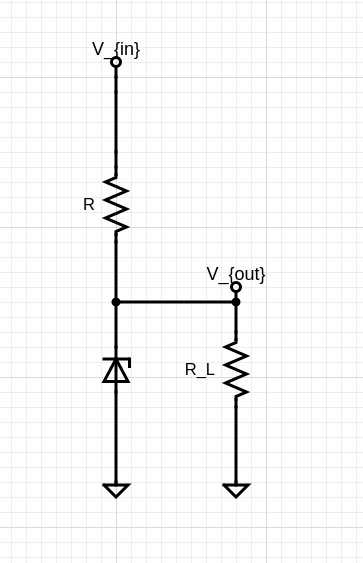
\includegraphics[width=0.3\textwidth]{q4}
    \caption{Circuit diagram for question 4. The diode is the 5.1-V IN5338B.}
    \label{fig:q4}
\end{figure}


\end{document}
